\documentclass{article}

\def\ParSkip{} 
% Packages
\usepackage{amssymb,amsmath,amsthm,bbm}
\usepackage{verbatim,float,url,dsfont}
\usepackage{graphicx,subfigure,psfrag}
\usepackage{algorithm,algorithmic}
\usepackage{mathtools,enumitem}
\usepackage{multirow}
\usepackage{ragged2e}
\usepackage{xr-hyper}
\usepackage{array}

\usepackage[colorlinks=true,citecolor=blue,urlcolor=blue,linkcolor=blue]{hyperref}
\usepackage[margin=1in]{geometry}
\usepackage[round]{natbib}

\usepackage[utf8]{inputenc} % allow utf-8 input
\usepackage[T1]{fontenc}    % use 8-bit T1 fonts
\usepackage{booktabs}       % professional-quality tables
\usepackage{nicefrac}         % compact symbols for 1/2, etc.
\usepackage{microtype}      % microtypography

\ifdefined\TimesFont 
\usepackage{times} % use times font
\fi

\ifdefined\ParSkip 
\usepackage{parskip} % use par skip
\fi

% Theorems and such
\newtheorem{theorem}{Theorem}
\newtheorem{lemma}{Lemma}
\newtheorem{corollary}{Corollary}
\newtheorem{proposition}{Proposition}
\theoremstyle{definition}
\newtheorem{remark}{Remark}
\newtheorem{definition}{Definition}

% Assumption
\newtheorem*{assumption*}{\assumptionnumber}
\providecommand{\assumptionnumber}{}
\makeatletter
\newenvironment{assumption}[2]{
  \renewcommand{\assumptionnumber}{Assumption #1#2}
  \begin{assumption*}
  \protected@edef\@currentlabel{#1#2}}
{\end{assumption*}}
\makeatother

% Widebar
\makeatletter
\newcommand*\rel@kern[1]{\kern#1\dimexpr\macc@kerna}
\newcommand*\widebar[1]{%
  \begingroup
  \def\mathaccent##1##2{%
    \rel@kern{0.8}%
    \overline{\rel@kern{-0.8}\macc@nucleus\rel@kern{0.2}}%
    \rel@kern{-0.2}%
  }%
  \macc@depth\@ne
  \let\math@bgroup\@empty \let\math@egroup\macc@set@skewchar
  \mathsurround\z@ \frozen@everymath{\mathgroup\macc@group\relax}%
  \macc@set@skewchar\relax
  \let\mathaccentV\macc@nested@a
  \macc@nested@a\relax111{#1}%
  \endgroup
}
\makeatother

% Min and max
\newcommand{\argmin}{\mathop{\mathrm{argmin}}}
\newcommand{\argmax}{\mathop{\mathrm{argmax}}}
\newcommand{\minimize}{\mathop{\mathrm{minimize}}}
\newcommand{\maximize}{\mathop{\mathrm{maximize}}}
\newcommand{\st}{\mathop{\mathrm{subject\,\,to}}}

% Shortcuts
\def\R{\mathbb{R}}
\def\C{\mathbb{C}}
\def\Z{\mathbb{Z}}
\def\N{\mathbb{N}}
\def\E{\mathbb{E}}
\def\P{\mathbb{P}}
\def\T{\mathsf{T}}
\def\Cov{\mathrm{Cov}}
\def\Var{\mathrm{Var}}
\def\indep{\perp\!\!\!\perp}
\def\th{^{\text{th}}}
\def\tr{\mathrm{tr}}
\def\df{\mathrm{df}}
\def\dim{\mathrm{dim}}
\def\col{\mathrm{col}}
\def\row{\mathrm{row}}
\def\nul{\mathrm{null}}
\def\rank{\mathrm{rank}}
\def\nuli{\mathrm{nullity}}
\def\spa{\mathrm{span}}
\def\sign{\mathrm{sign}}
\def\supp{\mathrm{supp}}
\def\diag{\mathrm{diag}}
\def\aff{\mathrm{aff}}
\def\conv{\mathrm{conv}}
\def\dom{\mathrm{dom}}
\def\hy{\hat{y}}
\def\hf{\hat{f}}
\def\hmu{\hat{\mu}}
\def\halpha{\hat{\alpha}}
\def\hbeta{\hat{\beta}}
\def\htheta{\hat{\theta}}
\def\cA{\mathcal{A}}
\def\cB{\mathcal{B}}
\def\cD{\mathcal{D}}
\def\cE{\mathcal{E}}
\def\cF{\mathcal{F}}
\def\cG{\mathcal{G}}
\def\cK{\mathcal{K}}
\def\cH{\mathcal{H}}
\def\cI{\mathcal{I}}
\def\cL{\mathcal{L}}
\def\cM{\mathcal{M}}
\def\cN{\mathcal{N}}
\def\cP{\mathcal{P}}
\def\cS{\mathcal{S}}
\def\cT{\mathcal{T}}
\def\cW{\mathcal{W}}
\def\cX{\mathcal{X}}
\def\cY{\mathcal{Y}}
\def\cZ{\mathcal{Z}}

\DeclareMathOperator*{\esssup}{ess\,sup}

\title{Supplementary Notes: B-Splines \\ \smallskip
\large Advanced Topics in Statistical Learning, Spring 2023 \\ \smallskip
Ryan Tibshirani}
\author{}
\date{}

\begin{document}
\maketitle
\RaggedRight
\vspace{-50pt}

Note: this is pretty much taken shamelessly from Appendix C of
\citet{tibshirani2022divided}.  

To parametrize the space of $k\th$ degree splines with knots at $t_1,\dots,t_r$,
a simple choice is the \emph{truncated power basis}, $g_1, \dots, g_{r+k+1}$,
which recall is defined as    
\begin{equation}
\begin{gathered}
\label{eq:tpb}
g_j(x) = \frac{1}{(j-1)!} x^{j-1}, \quad j=1,\dots,k+1, \\
g_{j+k+1}(x) = \frac{1}{k!} (x-t_j)^k_+, \quad j=1,\dots,r,
\end{gathered}
\end{equation}
Here $x_+=\max\{x,0\}$ denotes the positive part of $x$. 

Though the truncated power basis \eqref{eq:tpb} is the simplest basis for
splines, the B-spline basis is just as fundamental, and it was ``there at the 
very beginning'', appearing in Schoenberg's original paper on splines
\citep{schoenberg1946contributions1}. Here we are quoting
\citet{deboor1976splines}, who gives a masterful survey of the history and
properties of B-splines (and points out that the name ``B-spline'' is derived
from Schoenberg's use of the term ``basic spline'', to further advocate for the
idea that B-splines can be seen as \emph{the} basis for splines).

\paragraph{Peano representation.}

\def\st{^{\text{st}}}

There are different ways to construct B-splines; here we cover a construction
based on what is called the \emph{Peano representation} for B-splines. If $f$ is
a $k+1$ times differentiable function $f$ on an interval $[a,b]$ (and its
$(k+1)\st$ derivative is integrable), then by Taylor expansion
\[
f(z) = \sum_{i=0}^k \frac{1}{i!} (D^i f)(a) (z-a)^i + 
\int_a^z \frac{1}{k!} (D^{k+1} f)(x) (z-x)^k \, dx.
\]
Note that we can rewrite this as
\begin{equation}
\label{eq:taylor}
f(z) = \sum_{i=0}^k \frac{1}{i!} (D^i f)(a) (z-a)^i + 
\int_a^b \frac{1}{k!} (D^{k+1} f)(x) (z-x)^k_+ \, dx. 
\end{equation}

Next we will take a particular divided difference on both sides of the above
display. First we recall the definition of a divided difference: with respect to
two centers $z_1,z_2$, it is defined by       
\[
f[z_1,z_2] =  \frac{f(z_2)-f(z_1)}{z_2-z_1},
\]
and more generally, with respect to $k+1$ centers $z_1,\dots,z_{k+1}$, for an
integer $k \geq 1$, it is defined by  
\[
f[z_1,\dots,z_{k+1}] = \frac{f[z_2,\dots,z_{k+1}] -
f[z_1,\dots,z_k]}{z_{k+1}-z_1}.
\]
(For this to reduce to the definition with two centers, when $k=1$, we take by 
convention $f[z]=f(z)$.)   

Returning back to our main thread, we take a divided difference in the Taylor
expansion \eqref{eq:taylor} with respect to arbitrary centers $z_1,\dots,z_{k+2}
\in [a,b]$, where we assume without a loss of generality that $z_1 < \cdots <
z_{k+2}$, and then we use linearity to exchange divided differencing with
integration, yielding   
\begin{equation}
\label{eq:peano}
k! \cdot f[z_1,\dots,z_{k+2}] = \int_a^b (D^{k+1} f)(x)
\underbrace{(\cdot-x)^k_+[z_1,\dots,z_{k+2}]}_{P^k(x; z_{1:(k+2)})} \, dx, 
\end{equation}
where we have also used the fact that a $(k+1)\st$ order divided difference (with
respect to any $k+2$ centers) of a $k\th$ degree polynomial is zero, and we
multiplied both sides by $k!$. To be clear, the notation \smash{$(\cdot -
  x)^k_+[z_1,\dots,z_{k+2}]$} means that we are taking the divided difference of
the function \smash{$z \mapsto (z - x)^k_+$} with respect to centers
$z_1,\dots,z_{k+2}$.    

\paragraph{B-spline definition.}  

The result in \eqref{eq:peano} shows that the $(k+1)\st$ divided difference 
of any (smooth enough) function $f$ can be written as a weighted average of 
its $(k+1)\st$ derivative, in a local neighborhood around the corresponding
centers, where the weighting is given by a universal kernel \smash{$P^k(\cdot;
  z_{1:(k+2)})$} (that does not depend on $f$), which is called the \emph{Peano 
  kernel} formulation for the B-spline; to be explicit, this is
\[
P^k(x; z_{1:(k+2)}) = (\cdot - x)^k_+[z_1,\dots,z_{k+2}].
\]
Since 
\[
(z-x)^k_+ - (-1)^{k+1} (x-z)^k_+ =  (z-x)^k,
\]
and any $(k+1)\st$ order divided difference of the $k\th$ degree polynomial $z
\mapsto (z-x)^k$ is zero, we can rewrite the second-to-last display as
\[
P^k(x; z_{1:(k+2)}) = (-1)^{k+1} (x - \cdot)^k_+[z_1,\dots,z_{k+2}].
\]
The function \smash{$P^k(\cdot; z_{1:(k+2)})$} is called a $k\th$ degree
\emph{B-spline} with knots $z_{1:(k+2)}$. It is a linear combination of $k\th$ 
degree truncated power functions and is hence indeed a $k\th$ degree spline.  

It is often more convenient to deal with the \emph{normalized B-spline}:
\[
M^k(x; z_{1:(k+2)}) = (-1)^{k+1} (z_{k+2}-z_1) 
(x - \cdot)^k_+[z_1,\dots,z_{k+2}]. 
\]
It is easy to show that 
\[
\text{$M^k(\cdot; z_{1:(k+2)})$ is supported on $[z_1,z_{k+2}]$, and  
$M^k(x; z_{1:(k+2)})>0$ for $x \in (z_1,z_{k+2})$}.  
\]
To see the support result, note that for $x > z_{k+2}$, we are taking a divided
difference of all zeros, which of course zero, and for $x < z_1$, we are taking 
a $(k+1)\st$ order divided difference of a polynomial of degree $k$, which is
again zero. To see the positivity result, we can, for example, appeal to 
induction on $k$ and the recursion to come later.

\paragraph{B-spline basis.}  

To build a local basis the space of $k\th$ degree splines with knots
$t_1,\dots,t_r$, which we assume lie in the interior of $[a,b]$, we first define
boundary knots   
\[
t_{-k} < \cdots < t_{-1} < t_0 = a, \quad \text{and} \quad 
b = t_{r+1} < t_{r+2} < \cdots < t_{r+k+1}. 
\]
(Any such values for $t_{-k},\dots,t_0$ and $t_{r+1},\dots,t_{r+k+1}$ will
suffice to produce a basis; in fact, setting $t_{-k}=\cdots=t_0$ and
$t_{r+1}=\cdots=t_{r+k+1}$ would suffice, though this would require us to 
understand how to properly interpret divided differences with repeated centers;
as in Definition 2.49 of \citet{schumaker2007spline}.)  We then define the
normalized B-spline basis \smash{$M^k_j$}, $j=1,\dots,r+k+1$ 
\[
M^k_j = M^k(\cdot ; t_{(j-k-1):j}) \Big|_{[a,b]}, 
\quad j=1,\dots,r+k+1. 
\]
It is clear that each \smash{$M^k_j$}, $j=1,\dots,r+k+1$ is a $k\th$ degree    
spline with knots in $t_1,\dots,t_r$; hence to verify that they are a basis for
this space we only need to show their linear independence, which is
straightforward using the structure of their supports. 

For concreteness, we note that the $0\th$ degree normalized B-splines basis are
simply indicator functions,
\[
M^0_j = 1_{I_j}, \quad j=1,\dots,r+1.
\]
Here $I_0=[t_0,t_1]$ and $I_i=(t_i,t_{i+1}]$, $i=1,\dots,r$, and we use
$t_{r+1}=b$ for notational convenience. We note that this particular choice for
the half-open intervals (left- versus right-side open) is arbitrary, but
consistent with our definition of the truncated power basis \eqref{eq:tpb}
when $k=0$. 

Figure \ref{fig:bs} shows example normalized B-splines of degrees 0 through 3.    

\begin{figure}[tb]
\centering
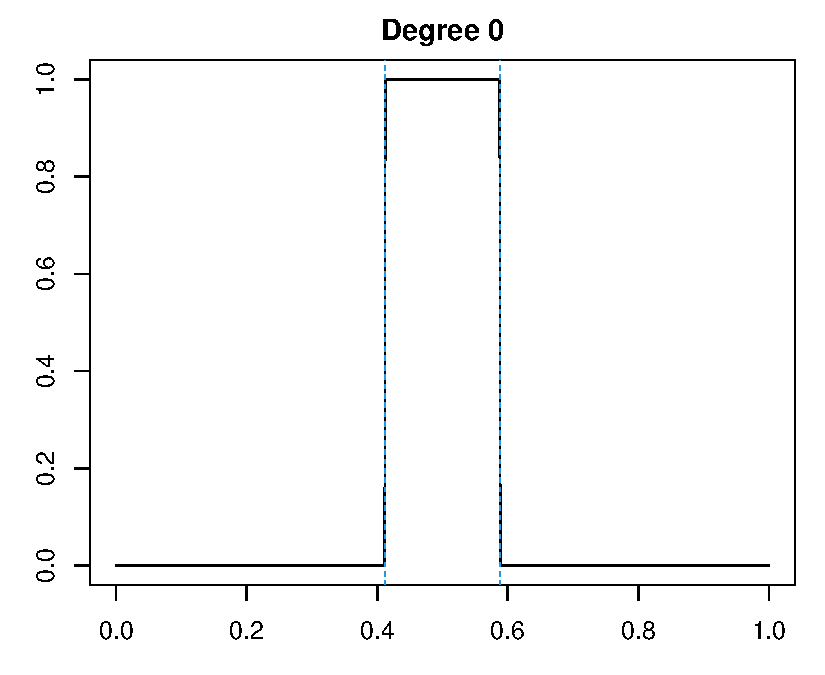
\includegraphics[width=0.475\textwidth]{bs0.pdf} 
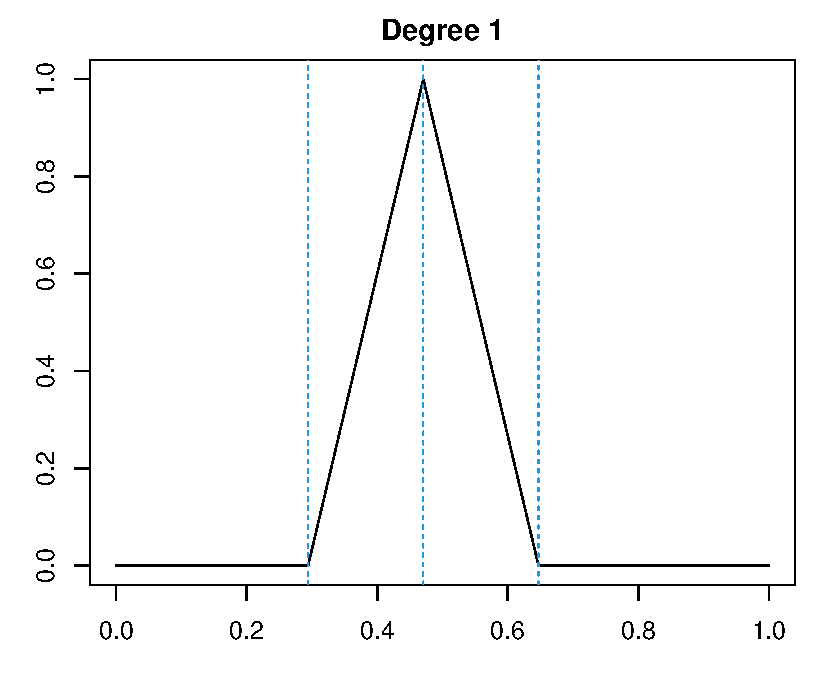
\includegraphics[width=0.475\textwidth]{bs1.pdf} 
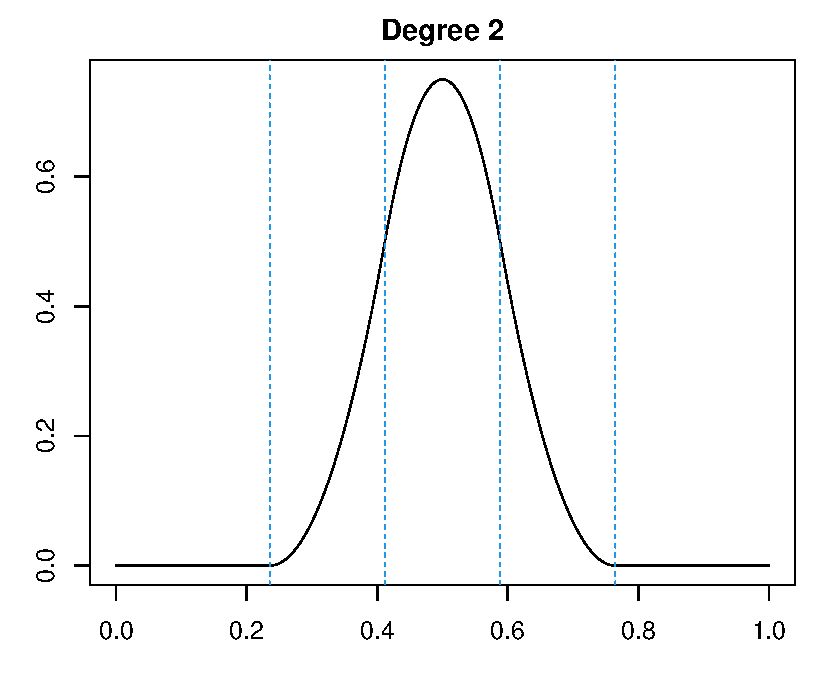
\includegraphics[width=0.475\textwidth]{bs2.pdf} 
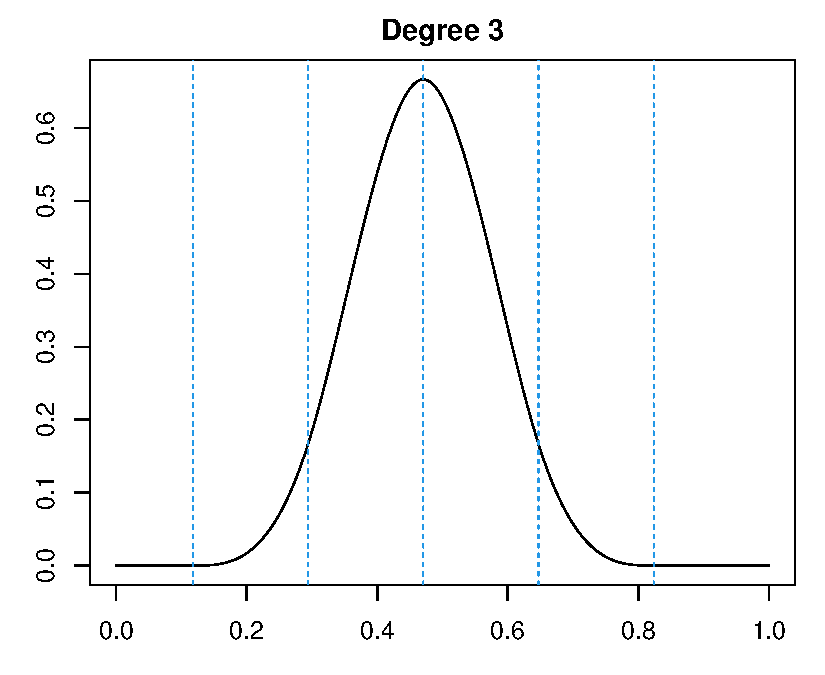
\includegraphics[width=0.475\textwidth]{bs3.pdf} 
\caption{\it B-splines of degrees 0 through 3. The knot points are marked by
  dashed blue vertical lines.}
\label{fig:bs}
\end{figure}

\paragraph{Recursive formulation.} 

B-splines satisfy a recursion relation that can be seen directly from the
recursive nature of divided differences: for any $k \geq 1$ and centers $z_1 <
\cdots < z_{k+2}$,  
\begin{align*}
(x - \cdot)^k_+ [z_1,\dots,z_{k+2}]
&= \frac{(x - \cdot)^k_+[z_2,\dots,z_{k+2}] - 
(x -\cdot)^k_+[z_1,\dots,z_{k+1}]}{z_{k+2} - z_1} \\
&= \frac{(x-z_{k+2})(x - \cdot)^{k-1}_+[z_2,\dots,z_{k+2}] 
- (x-z_1) (x - \cdot)^{k-1}_+[z_1,\dots,z_{k+1}] }{z_{k+2} - z_1},  
\end{align*} 
where in the second line we applied the Leibniz rule for divided differences 
\[
fg [z_1,\dots,z_{k+1}] = \sum_{i=1}^{k+1} f[z_1,\dots,z_i] g[z_i,\dots,z_{k+1}] 
\]
to conclude that
\begin{align*}
(x - \cdot)^k_+ [z_1,\dots,z_{k+1}] &= (x-z_1) \cdot 
(x - \cdot)^{k-1}_+ [z_1,\dots,z_{k+1}] \\
(x - \cdot)^k_+ [z_2,\dots,z_{k+2}] &= (x - \cdot)^{k-1}_+ 
  [z_2,\dots,z_{k+2}] \cdot (x-z_{k+2}). 
\end{align*}
Translating the above recursion over to normalized B-splines, we get 
\[
M^k(x; z_{1:(k+2)}) = \frac{x-z_1}{z_{k+1}-z_1} \cdot 
M^{k-1}(x; z_{1:(k+1)}) + \frac{z_{k+2}-x}{z_{k+2}-z_2} \cdot 
M^{k-1}(x; z_{2:(k+2)}),  
\]
which means that for the normalized basis, 
\[
M^k_j(x) = \frac{x-t_{j-k-1}}{t_{j-1}-t_{j-k-1}} \cdot
M^{k-1}_{j-1}(x) + \frac{t_j-x}{t_j-t_{j-k}} \cdot M^{k-1}_j(x), 
\quad j=1,\dots,r+k+1.  
\]
Above, we naturally interpret \smash{$M^{k-1}_0 = M^{k-1}(\cdot; 
  t_{-k:0})|_{[a,b]}$} and \smash{$M^{k-1}_{r+k+1} = M^{k-1}(\cdot;   
  t_{(r+1):(r+k+1)})|_{[a,b]}$}. 

The above recursions are very important, both for verifying numerous properties
of B-splines and for computational purposes. In fact, many authors prefer to
use recursion to define a B-spline basis in the first place.

\bibliographystyle{plainnat}
\bibliography{../../common/ryantibs.bib}

\end{document}